
\chapter{METODE PENENILITIAN}


\section{Tahapan Penelitian}
Tahapan dalam penelitian ini dapat dilihat pada gambar \ref{fig:penelitian-flowchart}.
\begin{afigure}
    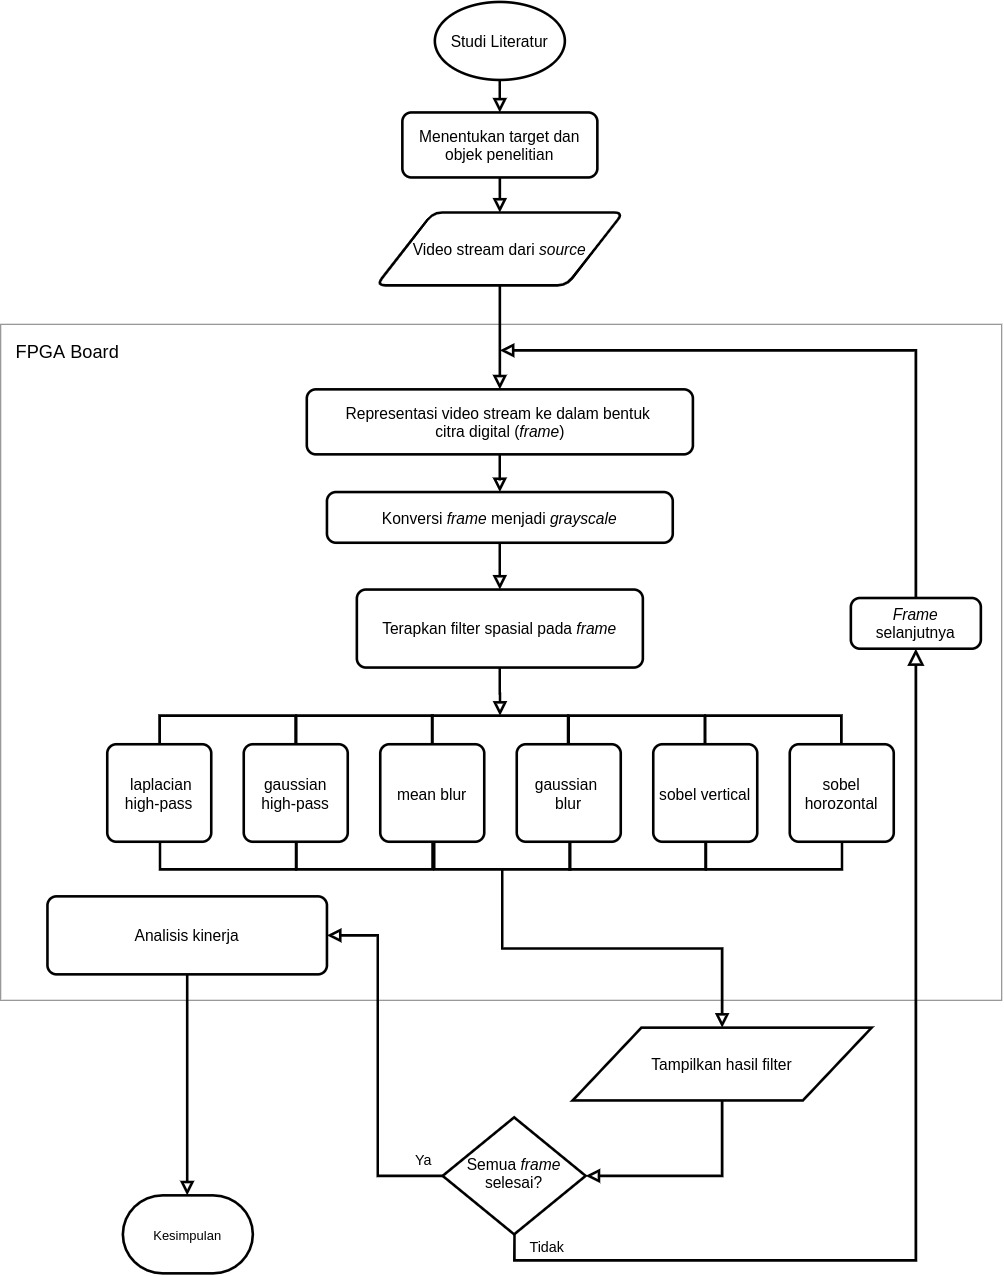
\includegraphics[width=13cm, center]{images/penelitian-flowchart.jpg}
    \caption{Flowchart tahapan penelitian.}
    \label{fig:penelitian-flowchart}
\end{afigure}
% tambahkan penjelasan lagi


\section{Waktu dan Lokasi Penelitian}
Penelitian ini dilaksanakan dari bulan Juni 2020 sampai dengan bulan Agustus 2020. Lokasi penelitian dilakukan di Laboratorium Rekayasa Perangkat Lunak Fakultas Matematika dan Ilmu Pengetahuan Alam, Universitas Hasanuddin Makassar.

\section{Rancangan Sistem}
Pada penelitian ini akan dibangun suatu sistem untuk mengimplementasikan filter spasial linear pada FPGA, dapat dilihat pada gambar \ref{fig:rancangan-sistem}.
\begin{afigure}
    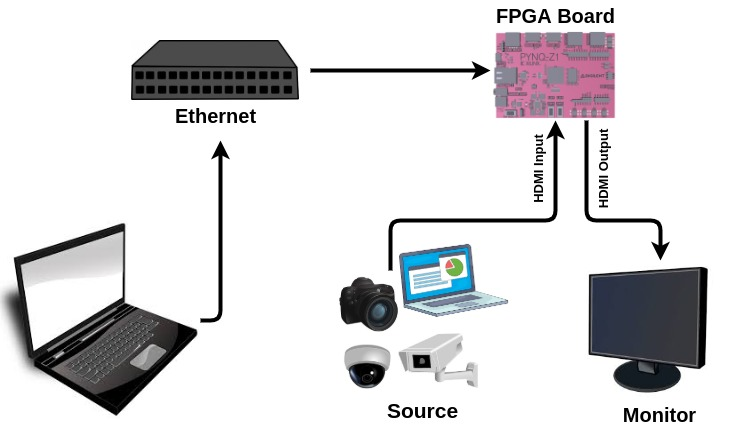
\includegraphics[width=0.85\textwidth, center]{images/rancangan-sistem.jpg}
    \caption{Rancangan sistem.}
    \label{fig:rancangan-sistem}
\end{afigure}

Video \textit{stream} dari \textit{source} disalurkan melalui port HDMI Input pada FPGA Development Board, kemudian video \textit{stream} tersebut akan diolah dengan menerapkan filter spasial linear pada setiap framenya. Setiap frame yang telah diterapkan filter spasial akan dialirkan ke monitor untuk kemudian ditampilkan. Selanjutnya dilakukan analisis kinerja pada FPGA. FPGA Development Board yang digunakan dalam penelitian ini dapat diakses dengan \textit{ssh} pada port 22 atau dengan Jupyter Notebook melalui browser.

\pagebreak

\section{Instrumen Penelitian}
\begin{enumerate}[topsep=0pt,itemsep=0pt,partopsep=0pt, parsep=0pt]
    \item Kebutuhan perangkat lunak:
    \begin{enumerate}[topsep=0pt,itemsep=0pt,partopsep=0pt, parsep=0pt, label={\alph*.}]
        \item Linux Ubuntu 18, sebagai OS pada FPGA Development Board.
        \item Python 3.6, dengan library OpenCV, Numpy, Pynq 5.2, dan Xilinx xfOpenCV.
        \item Jupyter Notebook pada FPGA Development Board. 
        \item Web Browser untuk mengakses Jupyter Notebook pada FPGA Development Board.
    \end{enumerate}
    \item Kebutuhan perangkat keras:
    \begin{enumerate}[topsep=0pt,itemsep=0pt,partopsep=0pt, parsep=0pt, label={\alph*.}]
        \item FPGA Development Board Xilinx PYNQ-Z2.
        \item Micro SD Card 16Gb, sebagai media penyimpanan OS pada FPGA Development Board.
        \item Monitor Eksternal, untuk menampilkan hasil penerapan filter spasial pada FPGA Development Board.
        \item Laptop Lenovo Ideapad 320 (sebagai \textit{source} video \textit{stream}).
    \end{enumerate}

    Spesifikasi FPGA Development Board yang digunakan:
    \begin{itemize}[topsep=0pt,itemsep=0pt,partopsep=0pt, parsep=0pt]
        \item Processor : Dual-Core ARM Cortex A9, 650 MHz
        \item FPGA : 1,3M reconfigurable gates
        \item Memory : 512 MB DDR3 / Flash
        \item Storage : Micro SD card slot
        \item Power : DC 7V-15V
        \item Dimension : 3,44" x 5,39" (87mm x 137mm)
    \end{itemize}
\end{enumerate}



